%%%%%%%%%%%%%%%%%%%%%%%
% Existing Approaches %
%%%%%%%%%%%%%%%%%%%%%%%

\chapter{Bestehende Ansätze für das Layout von Diagrammen}
\label{chapter:existing-approaches}

Dieses Kapitel widmet sich der Vorstellung von bestehenden Ansätzen für Layout von Diagrammen. Im Abschnitt \ref{sec:categorization} werden die Ansätze zunächst kategorisiert und anschließend werden in Abschnitten \ref{sec:manual-layout}, \ref{sec:automatic-layout} und \ref{sec:interactive-semi-automatic-layout} die einzelnen Hauptkategorien ausführlich beschrieben und deren Eigenschaften erläutert.

\section{Kategorisierung}
\label{sec:categorization}

Diese Arbeit setzt sich insbesondere mit der Interaktivität der Ansätze für das Layout von Diagrammen auseinander. Aus dem Grund werden die bestehenden Ansätze nach dem \textbf{Grad der Interaktivität} und der \textbf{Art der Layout-Unterstützung} in 3 Hauptkategorien unterteilt.

Zum einen gibt es das interaktive \textbf{manuelle Layout}, das auf der Freihand-Bearbeitung basiert und dem Nutzer ermöglicht, die Layout-Eigenschaften der Objekte im Diagramm wunschgemäß zu verändern, wobei dem Nutzer zusätzlich Layout-Vorschläge präsentiert werden. Das manuelle Layout wird in den meisten grafischen Editoren eingesetzt und wird näher im Abschnitt \ref{sec:manual-layout} erläutert.

Weiterhin gibt es Ansätze für das \textbf{vollautomatische Layout}, die optimale Layouts unter Berücksichtigung von ästhetischen Prinzipien produzieren. Sie haben einen statischen Charakter und können von dem Nutzer nur minimal beeinflusst werden. Somit sind sie nicht für interaktive Umgebungen geeignet. Mit diesen Ansätzen beschäftigt sich der Abschnitt \ref{sec:automatic-layout}.

Schließlich gibt es Ansätze für das \textbf{halbautomatische Layout}, die das Layout automatisiert berechnen, lassen sich aber durch den Nutzer interaktiv beeinflussen. Demzufolge kombinieren sie die Vorteile der vorigen beiden Kategorien. Diese Ansätze werden näher im Abschnitt \ref{sec:interactive-semi-automatic-layout} beschrieben.

\section{Manuelles Layout}
\label{sec:manual-layout}

In Anwendungen zum Erstellen von Diagrammen wie z.B. Vektorgrafik-Software, Präsentationsprogramme oder CASE-Tools wird ausschließlich das manuelle Layout unterstützt, d.h. die einzelnen Bestandteile können im Diagramm frei positioniert werden. Somit kann der Nutzer ein gewünschtes Layout erreichen, muss dafür aber viele manuelle Schritte tätigen \cite{Eichelberger05Aesthetics}. Da sich der Inhalt des Diagramms während der Erstellung ständig ändert, ist es notwendig, auch das Layout manuell anzupassen. Dies kann zur Frustration des Nutzers führen. Um einige Hürden des manuellen Layouts zu überwinden, bieten die Anwendungen eine Reihe an Funktionen, die dem Nutzer diese Tätigkeit bequemer machen.

Da das manuelle Layout auf direkter Interaktion des Nutzers mit dem Diagramm basiert, haben auch die Hilfefunktionen einen interaktiven Charakter. Außerdem weisen sie ein temporäres Verhalten auf, d.h. bei ihrer Nutzung werden keinerlei Regeln oder Constraints erstellt, wie das meistens bei den halbautomatischen Ansätzen der Fall ist (siehe Abschnitt \ref{sec:interactive-semi-automatic-layout}). Im Detail werden die Hilfefunktionen im Abschnitt \ref{subsec:help-functions-for-manual-layout} beschrieben.

\subsection{Anwendungen als Grundlage}
\label{subsec:applications-for-manual-layout}

Im Folgenden werden drei Anwendungen vorgestellt, an den die Hilfefunktionen für das manuelle Layout gezeigt werden.

\subsubsection{OmniGraffle}
\label{subsubsec:omnigraffle}

Die von \textit{OmniGroup}\footnote{\url{http://omnigroup.com}} entwickelte kommerzielle Anwendung \textit{OmniGraffle} ist eins der einfachsten Tools zur Erstellung von Diagrammen unter Mac OS X \cite{Olsen10OmniGraffle}. \textit{OmniGraffle} ist sehr flexibel und lässt sich für viele verschiedene Aufgaben einsetzen, z.B. von einem grafischen Entwurf einer Webseite bis zum Zeichnen von Klassendiagrammen. Das liegt vor allem daran, dass für die gezeichneten Diagramme kein semantisches Modell vorliegt und dass die Diagrammbestandteile als reine vektorgrafische Objekte repräsentiert werden. Detaillierte Informationen zu \textit{OmniGraffle} können in \cite{08OmniGraffle}, \cite{Olsen10OmniGraffle} oder auf der offiziellen Webseite\footnote{\url{http://omnigroup.com/omnigraffle}} gefunden werden.

Die meisten im Abschnitt \ref{subsec:help-functions-for-manual-layout} beschriebenen Hilfefunktionen für das manuelle Layout werden anhand von \textit{OmniGraffle} 5\footnote{Die aktuelle Version von \textit{OmniGraffle} ist 6 (\url{http://www.omnigroup.com/blog/omnigraffle-6-is-here}), die Erkenntnisse für diese Arbeit wurden allerdings mit der Version 5 gewonnen.} gezeigt. \textit{OmniGraffle} bietet auch eine Unterstützung für automatisches Layout, die näher im Abschnitt \ref{subsubsec:omnigraffle-auto-layout} beschrieben wird.

\subsubsection{Keynote}
\label{subsubsec:keynote}

\textit{Apple} \textit{Keynote} ist eine Anwendung zur Erstellung von Präsentationen für Mac OS X und iOS. Es bietet ähnliche Funktionen wie Microsoft PowerPoint\footnote{\url{http://office.microsoft.com/en-us/powerpoint/}} und bildet somit eine Alternative zu dem bekannten Präsentationsprogramm. Neben den Achsendiagrammen zur Visualisierung von Werten wie Linien- oder Balkendiagramme ermöglicht \textit{Keynote} mit Hilfe von vektorgrafischen Objekten einfache graphbasierte Diagramme zu erstellen. Weitere Informationen sind in \cite{11Keynote} oder auf der offiziellen Webseite\footnote{\url{http://www.apple.com/de/mac/keynote/}} zu finden. 

\textit{Keynote} besitzt ähnliche oder sogar identische Hilfefunktionen für das manuelle Layout wie \textit{OmniGraffle}. Im Abschnitt \ref{subsec:help-functions-for-manual-layout} werden einige Hilfefunktionen anhand von \textit{Keynote} 6 erklärt. Das automatische Layout wird in \textit{Keynote} nicht unterstützt.

\subsubsection{Visual Paradigm}
\label{subsubsec:visual-paradigm}

\textit{Visual Paradigm} ist ein plattformunabhängiges CASE-Tool von der gleichnamigen Firma und unterstützt neben UML-Diagrammen auch weitere visuelle Sprachen \cite{14Visual}. Das Tool basiert auf einer Freihandbearbeitung und bietet neben Hilfefunktionen für das manuelle Layout (siehe Abschnitt \ref{subsec:help-functions-for-manual-layout}) auch Unterstützung für automatische Layout-Algorithmen (siehe Abschnitt \ref{subsec:visual-approaches}) \cite{Fuhrmann11On-the-Pragmatics}. Mit der näheren Beschreibung von \textit{Visual Paradigm} beschäftigen sich \cite{14Visual}, \cite[S.313-314]{Fuhrmann11On-the-Pragmatics} und die offizielle Webseite\footnote{\url{http://www.visual-paradigm.com}}.

\subsection{Hilfefunktionen für manuelles Layout}
\label{subsec:help-functions-for-manual-layout}

\subsubsection{Raster}
\label{subsubsec:grid}

Viele (unter anderem alle drei im Abschnitt \ref{subsec:applications-for-manual-layout} erwähnten) Visualisierungsprogramme unterstützen die Aufteilung des Diagramms in ein gleichmäßiges Raster, das durch Rasterlinien dargestellt werden kann. Diese Linien können zum Ausrichten von Objekten im Diagramm verwendet werden, das vor allem dann nützlich ist, wenn die Größen der Objekte eine wichtige Rolle spielen wie z.B. Grundrisse \cite{08OmniGraffle, Olsen10OmniGraffle, 11Keynote, 14Visual}.

\paragraph{Snap-to-Grid}

Die reguläre Verschiebungsoperation von Objekten im Diagramm funktioniert in der Regel wie folgt: Der Nutzer wählt mit dem Mauszeiger ein Objekt aus und schiebt das Objekt mit gedrückter Maustaste auf seine neue Position. Wenn die Funktion \enquote{Snap-to-Grid} nicht aktiviert ist, kann die Zielposition beliebig sein. Während der Verschiebung wird die Position des Objekts kontinuierlich angepasst, so dass der Nutzer ein visuelles Feedback bekommt. Dieser Vorgang ist in Abbildung \ref{fig:omnigraffle-snap-to-grid-off} dargestellt.

\begin{figure}[hbt]
    \newcommand{\subfigurewidth}{0.33\textwidth}
    \newcommand{\graphicswidth}{0.95\linewidth}
    \begin{subfigure}{\subfigurewidth}
        \centering
        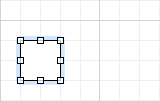
\includegraphics[width=\graphicswidth]{resources/omnigraffle-snap-to-grid-off-a}
        \caption{}
    \end{subfigure}
    \begin{subfigure}{\subfigurewidth}
        \centering
        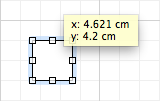
\includegraphics[width=\graphicswidth]{resources/omnigraffle-snap-to-grid-off-b}
        \caption{}
    \end{subfigure}
    \begin{subfigure}{\subfigurewidth}
        \centering
        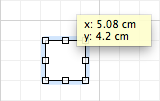
\includegraphics[width=\graphicswidth]{resources/omnigraffle-snap-to-grid-off-c}
        \caption{}
    \end{subfigure}
    \caption{Verschiebungsoperation mit nicht aktivierter Funktion \enquote{Snap-to-Grid} in \textit{OmniGraffle}}
    \label{fig:omnigraffle-snap-to-grid-off}
\end{figure}

Wenn die Funktion \enquote{Snap-to-Grid} nun aktiviert ist, wird im Unterschied zu dem vorigen Vorgang die Zielposition so eingeschränkt, dass das verschobene Objekt an den Rasterlinien ausgerichtet wird. Der Mauszeiger kann dabei frei positioniert werden, das Objekt nimmt aber immer die nächste ausgerichtete Position an. Dieser Vorgang ist in Abbildung \ref{fig:omnigraffle-snap-to-grid-on} dargestellt.

\begin{figure}[hbt]
    \newcommand{\subfigurewidth}{0.33\textwidth}
    \newcommand{\graphicswidth}{0.95\linewidth}
    \begin{subfigure}{\subfigurewidth}
        \centering
        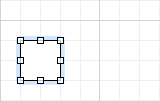
\includegraphics[width=\graphicswidth]{resources/omnigraffle-snap-to-grid-on-a}
        \caption{}
    \end{subfigure}
    \begin{subfigure}{\subfigurewidth}
        \centering
        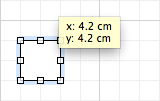
\includegraphics[width=\graphicswidth]{resources/omnigraffle-snap-to-grid-on-b}
        \caption{}
    \end{subfigure}
    \begin{subfigure}{\subfigurewidth}
        \centering
        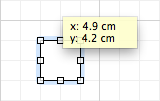
\includegraphics[width=\graphicswidth]{resources/omnigraffle-snap-to-grid-on-c}
        \caption{}
    \end{subfigure}
    \caption{Verschiebungsoperation mit aktivierter Funktion \enquote{Snap-to-Grid} in \textit{OmniGraffle}}
    \label{fig:omnigraffle-snap-to-grid-on}
\end{figure}

Neben der Verschiebungsoperation wird auch die Operation der Größenänderung eingeschränkt, indem das manipulierte Objekt nur so eine Größe annehmen kann, die die Ausrichtung an die Rasterlinien nicht verletzt.

\paragraph{Ausrichten im Raster}

Das Ausrichten an Rasterlinien kann auch nachträglich bewirkt werden. Dies passiert durch die Auswahl des auszurichtenden Objekts und dem Ausführen der Funktion \textit{Ausrichten im Raster}. Die Position und Größe des Objekts werden so angepasst, dass das Objekt an den Rasterlinien ausgerichtet wird.

\subsubsection{Ausrichten und Verteilen von Objekten in Relation zueinander}
\label{subsubsec:alignment-and-distribution}

Ähnlich wie das Raster (Abschnitt \ref{subsubsec:grid}) werden die Funktionen zum Ausrichten und Verteilen von ausgewählten Objekten häufig in Visualisierungsprogrammen eingesetzt. Sie funktionieren wie folgt: Der Nutzer wählt im Diagramm Objekte aus, auf die die Funktion angewendet werden soll. Nachher wählt er eine konkrete Form der Funktion aus, die anschließend auf die ausgewählten Objekt angewendet wird \cite{11Keynote}.

\paragraph{Ausrichten}

Die ausgewählten Objekte können in Relation zueinander ausgerichtet werden. Dafür muss nach der Auswahl von mindestens 2 Objekten die Form der Ausrichtung angegeben werden. Die Objekte können entweder vertikal (linke Kanten, Mittelpunkte oder rechte Kanten) oder horizontal (obere Kanten, Mittelpunkte oder untere Kanten) ausgerichtet werden. Nach dem Ausführen dieser Funktion werden die Positionen der ausgewählten Objekte so angepasst, dass die gewünschte Ausrichtung erfüllt ist \cite{11Keynote, 08OmniGraffle}. Ein Beispiel ist in Abbildung \ref{fig:keynote-horizontal-alignment} zu finden.

\begin{figure}[hbt]
    \newcommand{\subfigurewidth}{0.5\textwidth}
    \begin{subfigure}{\subfigurewidth}
        \centering
        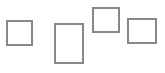
\includegraphics{resources/keynote-horizontal-alignment-a}
        \caption{}
    \end{subfigure}
    \begin{subfigure}{\subfigurewidth}
        \centering
        
\includegraphics{resources/keynote-horizontal-alignment-b}
        \caption{}
    \end{subfigure}
    \caption{Anwendung der horizontalen zentrierten Ausrichtung in \textit{Keynote}}
    \label{fig:keynote-horizontal-alignment}
\end{figure}

\paragraph{Verteilen}

Wenn mindestens 3 Objekte ausgewählt werden, kann die Funktion zum gleichmäßigen Verteilen der Objekte angewendet werden. Dabei wird die Position der äußeren Objekte fixiert und die Position von umschlossenen Objekten wird so angepasst, dass die vertikalen bzw. horizontalen Abstände zwischen den Objekten gleich sind (siehe Abbildung \ref{fig:keynote-horizontal-distribution}) \cite{11Keynote}.

\begin{figure}[hbt]
    \newcommand{\subfigurewidth}{0.5\textwidth}
    \begin{subfigure}{\subfigurewidth}
        \centering
        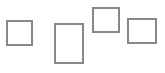
\includegraphics{resources/keynote-horizontal-distribution-a}
        \caption{}
    \end{subfigure}
    \begin{subfigure}{\subfigurewidth}
        \centering
        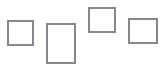
\includegraphics{resources/keynote-horizontal-distribution-b}
        \caption{}
    \end{subfigure}
    \caption{Anwendung der horizontalen Verteilung in \textit{Keynote}}
    \label{fig:keynote-horizontal-distribution}
\end{figure}

\subsubsection{Smart Guides}
\label{subsubsec:smart-guides}

Eine sehr hilfreiche Funktion, die in den meisten Grafik- und Präsentationsprogrammen unterstützt wird, sind Hilfslinien für Ausrichtung und relative Positionierung (engl. \textit{Smart Guides}) \cite{11Keynote}. Wenn diese Funktion aktiviert ist, werden während der Manipulation des ausgewählten Objekts farbige Linien im Canvas eingeblendet. Diese Linien geben dem Nutzer ein visuelles Feedback zur geeigneten Ausrichtung des manipulierten Objekts relativ zu anderen Objekten im Diagramm. Außerdem wird ähnlich wie bei der Funktion \textit{Snap-to-Grid} die freie Manipulation eingeschränkt, was in der Regel zu besseren Layout-Ergebnissen führt. Die Hilfslinien werden nach der Beendigung der Operation wieder ausgeblendet und die Position bzw. Größe des manipulierten Objektes wird angepasst. Genauso wie auch bei allen anderen Hilfefunktionen für das manuelle Layout handelt es sich bei den Hilfslinien um eine temporäre Layout-Funktion. Somit wird die Ausrichtung der Objekte nur in den Eigenschaften der Objekte (Position und Größe) ausgedrückt und es wird keine explizite Regel erstellt.

\paragraph{Hilfslinien zur Ausrichtung (Alignment Guides)}

Die erste Art der Hilfslinien ist für die Ausrichtung des verschobenen Objekts an den Kanten bzw. Mittelachsen von anderen Objekten in Diagram nützlich. Die Linien werden während der Verschiebungsoperation eingeblendet, wenn das verschobene Objekt an ein anderes Objekt ausgerichtet wird \cite{11Keynote}.

\begin{figure}[hbt]
    \newcommand{\subfigurewidth}{0.5\textwidth}
    \begin{subfigure}{\subfigurewidth}
        \centering
        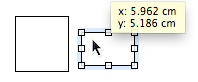
\includegraphics{resources/omnigraffle-smart-guides-a}
        \caption{}
        \label{fig:omnigraffle-smart-guides-a}
    \end{subfigure}
    \begin{subfigure}{\subfigurewidth}
        \centering
        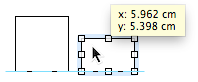
\includegraphics{resources/omnigraffle-smart-guides-b}
        \caption{}
        \label{fig:omnigraffle-smart-guides-b}
    \end{subfigure}
    \begin{subfigure}{\subfigurewidth}
        \centering
        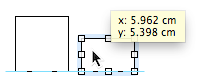
\includegraphics{resources/omnigraffle-smart-guides-c}
        \caption{}
        \label{fig:omnigraffle-smart-guides-c}
    \end{subfigure}
    \begin{subfigure}{\subfigurewidth}
        \centering
        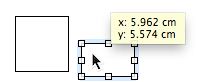
\includegraphics{resources/omnigraffle-smart-guides-d}
        \caption{}
        \label{fig:omnigraffle-smart-guides-d}
    \end{subfigure}
    \caption{Hilfslinien zur Ausrichtung während der Verschiebungsoperation in \textit{OmniGraffle}}
    \label{fig:omnigraffle-smart-guides}
\end{figure}

In Abbildung \ref{fig:omnigraffle-smart-guides} wird ein Beispiel der Hilfslinien zur Ausrichtung der unteren Kanten von 2 Objekten während einer Verschiebungsoperation veranschaulicht. Zunächst wird in \ref{fig:omnigraffle-smart-guides-a} das rechte Objekt ausgewählt und nach unten verschoben. Wenn sich die untere Kante des verschobenen Objekts der unteren Kante des inaktiven Objekts nähert, so wie es in \ref{fig:omnigraffle-smart-guides-b} der Fall ist, wird eine Hilfslinie eingeblendet und das verschobene Objekt springt auf eine ausgerichtete Position hin. In \ref{fig:omnigraffle-smart-guides-c} wird die Verschiebung weitergeführt, das anhand der Position des Mauszeigers erkannt werden kann. Das Objekt bleibt so lange ausgerichtet, bis der Abstand der Kanten eine bestimmte Schwelle in \ref{fig:omnigraffle-smart-guides-d} überschreitet. Danach wird die Hilfslinie ausgeblendet und eine freie Positionierung ist wieder möglich.

Aus dem vorgestellten Beispiel folgt, dass sich um die untere Kante des inaktiven Objekts ein Bereich bildet, in dem das verschobene Objekt auf die ausgerichtete Position hinspringt. Dies passiert, wenn sich die Geraden in der Nähe befinden und der Abstand unter einer bestimmten Schwelle liegt. Dieser Bereich wird in Abbildung \ref{fig:omnigraffle-smart-guides-snap-area} visualisiert.

\begin{figure}[hbt]
    \centering
    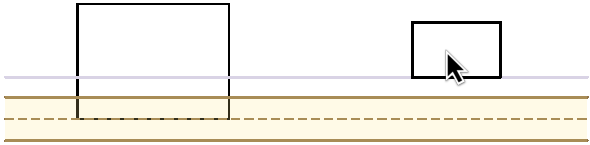
\includegraphics{resources/omnigraffle-smart-guides-snap-area}
    \caption{Visualisierung des Bereichs für die Ausrichtung an die untere Kante des linken Objekts}
    \label{fig:omnigraffle-smart-guides-snap-area}
\end{figure}

Solche Bereiche werden für alle Kanten und Mittelachsen von nicht ausgewählten Objekten in der horizontalen und vertikalen Richtung gebildet. Wenn der Nutzer ein Objekt verschiebt und eine der Kanten oder die Mittelachse des verschobenen Objekts sich in einem der Bereiche befindet, wird seine Position ausgerichtet, ohne den Mauszeiger zu beeinflussen. Das kann auch gleichzeitig für die horizontale und vertikale Richtung der Fall sein. Somit kann z.B. ein Objekt in einem anderen Objekt zentriert werden (siehe Abbildung \ref{fig:omnigraffle-alignment-guides-centering}).

\begin{figure}[hbt]
    \centering
    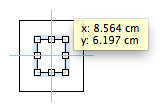
\includegraphics{resources/omnigraffle-alignment-guides-centering.png}
    \caption{Ausrichten eines Objekts in einem anderen Objekt mit Hilfe von einer horizontalen und einer vertikalen Hilfslinie zur Ausrichtung in \textit{OmniGraffle}}
    \label{fig:omnigraffle-alignment-guides-centering}
\end{figure}

Eine Veranschaulichung dieser Funktion bietet in Form einer JavaScript-Anwendung das Open-Source Projekt \textit{Alignment-Guides}\footnote{Quellcode: \url{https://github.com/mrflix/Alignment-Guides}, Demo-Anwendung: \url{http://mrflix.github.io/Alignment-Guides}}.

\paragraph{Abstandshilfslinien (Distance Guides)}

Die zweite Art der Hilfslinien dient dazu, die Abstände zwischen 3 Objekten in einer horizontalen oder vertikalen Reihe gleich zu halten. Während der Verschiebung eines der 3 Objekten wird ein Bereich gebildet, in dem das Objekt zu der Position hinspringt, in der die Abstände zwischen den einzelnen Objektpaaren gleich sind. Zusätzlich zu den Hilfslinien wird auch der Abstand eingeblendet \cite{11Keynote, Olsen10OmniGraffle}.

\begin{figure}[hbt]
    \centering
    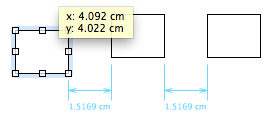
\includegraphics{resources/omnigraffle-distance-guides.png}
    \caption{Abstandshilfslinien in \textit{OmniGraffle}}
    \label{fig:omnigraffle-distance-guides}
\end{figure}

\paragraph{Größenhilfslinien (Sizing Guides)}

Im Unterschied zu den zwei vorigen Arten der Hilfslinien wird die letzte Art durch die Operation der Größenänderung eines Objektes hervorgerufen. Wenn sich die Größe des manipulierten Objekts der Größe eines anderen Objekts im Diagramm nähert und die Differenz unter einer bestimmten Grenze liegt, wird die Größe des anderen Objekts übernommen. Dies funktioniert getrennt für die Breite und Höhe (siehe Abbildung \ref{fig:omnigraffle-sizing-guides}).

\begin{figure}[hbt]
    \centering
    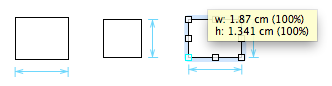
\includegraphics{resources/omnigraffle-sizing-guides.png}
    \caption{Größenhilfslinien in \textit{OmniGraffle}}
    \label{fig:omnigraffle-sizing-guides}
\end{figure}

\subsubsection{Manuelle Hilfslinien}

Weiterhin bieten \textit{OmniGraffle} und \textit{Keynote} die Funktion der Erstellung von manuellen Hilfslinien an \cite{08OmniGraffle, 11Keynote}. Diese Funktion ist sehr ähnlich zu \textit{Smart Guides}, unterscheidet sich aber wie folgt:

\begin{itemize}
    \item Die Hilfslinien werden vom Nutzer manuell platziert - entweder horizontal oder vertikal.
    \item Die Hilfslinien sind global für das gesamte Diagramm und damit nicht relativ zu einem anderen Objekt im Diagramm.
    \item Die Hilfslinien sind permanent sichtbar, auch wenn keine Verschiebungsoperation stattfindet.\footnote{Die Anzeige der manuellen Hilfslinien kann sowohl in \textit{OmniGraffle} als auch in \textit{Keynote} global aus- und eingeschaltet werden.}
\end{itemize}

Die Gemeinsamkeit besteht darin, dass das Ausrichten an die Hilfslinien identisch wie bei den \textit{Smart Guides} funktioniert (siehe Abschnitt \ref{subsubsec:smart-guides}). Ein Bespiel der manuellen Hilfslinie in \textit{OmniGraffle} wird in Abbildung \ref{fig:omnigraffle-manual-guides} dargestellt.

\begin{figure}[hbt]
    \centering
    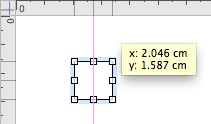
\includegraphics{resources/omnigraffle-manual-guides.png}
    \caption{Beispiel einer manuellen Hilfslinie in \textit{OmniGraffle}}
    \label{fig:omnigraffle-manual-guides}
\end{figure}

Wie bereits erwähnt, ist das Ausrichten an die manuellen Hilfslinien nicht persistent und eine Verschiebung der Hilfslinie verursacht keine Verschiebung der ausgerichteten Objekte. Dieses Verhalten wird allerdings in den Tool Microsoft Visio\footnote{\url{http://visio.microsoft.com}} und ConceptDraw\footnote{\url{http://conceptdraw.com}} unterstützt und wird mit Hilfe von Einweg-Constraints realisiert \cite[S.20]{Maier12A-Pattern-based}.

\subsubsection{Gleiche Größe der Objekte}

Sehr trivial, aber dennoch nützlich ist die Funktion der Einstellung von gleichen Größen für ausgewählte Objekte. Nach der Auswahl von 2 oder mehreren Objekten im Diagramm hat der Nutzer die Möglichkeit, die Breite, die Höhe oder beide Dimensionen gleichzeitig auf die Werte des zuerst ausgewählten Objektes zu setzen (siehe Abbildung \ref{fig:omnigraffle-make-same-size}). Diese Funktion wird in \textit{OmniGraffle} unterstützt \cite{Olsen10OmniGraffle}.

\begin{figure}[hbt]
    \newcommand{\subfigurewidth}{0.5\textwidth}
    \begin{subfigure}{\subfigurewidth}
        \centering
        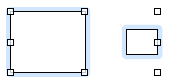
\includegraphics{resources/omnigraffle-make-same-size-a}
        \caption{}
        \label{fig:omnigraffle-make-same-size-a}
    \end{subfigure}
    \begin{subfigure}{\subfigurewidth}
        \centering
        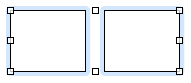
\includegraphics{resources/omnigraffle-make-same-size-b}
        \caption{}
        \label{fig:omnigraffle-make-same-size-b}
    \end{subfigure}
    \caption{Anwendung der Funktion zur Einstellung von gleichen Größen in \textit{OmniGraffle}}
    \label{fig:omnigraffle-make-same-size}
\end{figure}

\subsubsection{Verknüpfungspunkte für Verbindungen}
\label{subsubsec:connection-points}

Die bisher diskutierten Hilfefunktionen haben sich ausschließlich mit der Positionierung und Bestimmung der Größe der Objekte auseinandergesetzt. Für die graphbasierten Diagramme (siehe Abschnitt \ref{subsec:graph-based-diagrams}) sind neben der Knoten auch Kanten von Interesse, die in der Regel durch Verbindungslinien dargestellt werden. Wenn 2 Objekte mit einer Verbindungslinie verbunden werden, bleiben sie auch dann verbunden, wenn sich die Position oder Größe der Objekte ändert \cite{11Keynote}. In vielen Programmen (unter anderem in \textit{Keynote} und \textit{OmniGraffle}) werden die Verknüpfungspunkte der Verbindungslinie standardmäßig an die Stellen positioniert, an den eine gedachte Strecke, die die Mittelpunkte beider Objekte verbindet, die Kanten der Objekte schneidet (siehe Abbildung \ref{fig:omnigraffle-connection-points}) \cite{08OmniGraffle}.

\begin{figure}[hbt]
    \newcommand{\subfigurewidth}{0.5\textwidth}
    \newcommand{\graphicswidth}{0.8\linewidth}
    \begin{subfigure}{\subfigurewidth}
        \centering
        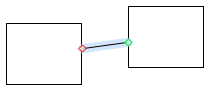
\includegraphics[width=\graphicswidth]{resources/omnigraffle-connection-points-a}
        \caption{}
        \label{fig:omnigraffle-connection-points-a}
    \end{subfigure}
    \begin{subfigure}{\subfigurewidth}
        \centering
        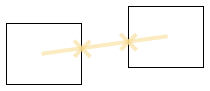
\includegraphics[width=\graphicswidth]{resources/omnigraffle-connection-points-b}
        \caption{}
        \label{fig:omnigraffle-connection-points-b}
    \end{subfigure}
    \caption{Verknüpfungspunkte einer Verbindung in \textit{OmniGraffle} \subref{fig:omnigraffle-connection-points-a} mit Veranschaulichung der Berechnung \subref{fig:omnigraffle-connection-points-b}}
    \label{fig:omnigraffle-connection-points}
\end{figure}

\textit{OmniGraffle} bietet die Möglichkeit, mit Hilfe des Magnetwerkzeugs manuell die Verknüpfungspunkte zu definieren. Dies funktioniert auf zwei verschiedene Arten. Entweder kann der Nutzer die Verknüpfungspunkte beliebig in dem Objekt positionieren oder er wählt eine vordefinierte Anordnung aus. Dazu gehören u.a. die gleichmäßige Verteilung einer festen Anzahl an Verknüpfungspunkten entlang allen Kanten oder die Positionierung eines Verknüpfungspunktes an jedem Eckpunkt. Ein Beispiel der Darstellung von Verknüpfungspunkten ist in Abbildung \ref{fig:omnigraffle-magnets-example} zu finden.

\begin{figure}[hbt]
    \centering
    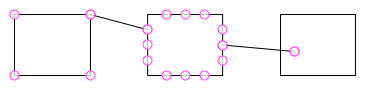
\includegraphics{resources/omnigraffle-magnets-example.png}
    \caption{Beispiel der manuellen Verknüpfungspunkte in \textit{OmniGraffle}: Magnete an den Eckpunkten (links), 3 Magnete pro Kante (Mitte), ein manuell positionierter Magnet (rechts)}
    \label{fig:omnigraffle-magnets-example}
\end{figure}

Sobald mindestens ein Magnet dem Objekt hinzugefügt wurde, wird nicht mehr der Verknüpfungspunkt mit Hilfe des Mittelpunktes berechnet wie oben beschrieben, sondern die Verbindungslinie wird immer von dem nächsten Verknüpfungspunkt angezogen (siehe Abbildung \ref{fig:omnigraffle-magnets-example}). Alternativ kann der Nutzer ein Ende der Verbindungslinie an einen konkreten Verknüpfungspunkt binden. In dem Fall bleibt die Verbindungslinie an den gewählten Verknüpfungspunkt gebunden, auch wenn ein anderer Verknüpfungspunkt näher ist.

\subsection{Zusammenfassung der Eigenschaften}

\subsubsection{Vorteile}

\begin{itemize}
    \item \textbf{Interaktion} Das manuelle Layout stellt die Interaktion des Nutzers mit dem Diagramm in den Vordergrund und ist dadurch sehr intuitiv.
    \item \textbf{Flexibilität} Aufgrund der Möglichkeit der beliebigen Anpassung der Layout-Eigenschaften kann das manuelle Layout sehr präzis gesteuert werden. Somit hat der Nutzer einen großen Einfluss auf das resultierende Layout.
\end{itemize}

\subsubsection{Nachteile}

\begin{itemize}
    \item \textbf{Fehlende Unterstützung der Diagrammtypen} Die Tools, die das manuelle Layout einsetzen, lassen sich in zwei Gruppen unterteilen: CASE-Tools, die die grafische Notation der Diagrammtypen unterstützen und Vektorgrafik-Tools, die eine geringe bis keine Unterstützung der grafischen Notation bringen. Jedoch werden die Syntax- und Semantikregeln für die Layout-Erstellung weder in den CASE-Tools noch in den Vektorgrafik-Tools berücksichtigt und können durch den Nutzer verletzt werden.    
    \item \textbf{Aufwand an Layout-Erstellung} Die Aktionen zur Erstellung des Layouts sind temporär und nach jeder Änderung des Inhalts eines Diagramms muss das erstellte Layout neu angepasst werden, das in der Regel mit viel Aufwand verbunden ist.
\end{itemize}

\section{Automatisches Layout}
\label{sec:automatic-layout}

Den graphbasierten Softwarediagrammen unterliegt die abstrakte Struktur des Graphen (siehe Abschnitt \ref{subsec:graph-based-diagrams}). Mit der grafischen Darstellung von Graphen beschäftigt sich die mathematische Disziplin des Graphzeichnens. Ihre Aufgabe besteht darin, Layout-Algorithmen zu entwerfen, die optimale Layouts in Hinsicht auf ästhetische Regeln erzeugen, d.h. die Layout-Eigenschaften wie Position der Knoten und Routen der Kanten berechnen \cite{Eichelberger05Aesthetics, Arvo02Techniques, Siebenhaller03Automatisches, Maier12A-Pattern-based}. Unter dem automatischen Layout für graphbasierte Diagramme sind daher vollautomatische Algorithmen zu verstehen, die für ein gegebenes Diagramm die optimalen Layout-Eigenschaften berechnen und das Diagramm entsprechend anpassen \cite{Fuhrmann11On-the-Pragmatics}.

Um während der Erstellung des Diagramms immer ein optimales Layout zu erhalten, muss der Layout-Algorithmus kontinuierlich nach jeder Änderung des Inhalts entweder automatisch oder manuell aufgerufen werden. Wenn eine Interaktion mit dem resultierenden Diagramm unterstützt wird, hat sie keinerlei Einwirkung auf den Algorithmus und wird bei dem nächsten Aufruf nicht berücksichtigt. In der Regel kann der Nutzer nur bestimmte Parameter des Algorithmus\footnote{z.B. minimale Länge der Kanten im zirkulären Layout-Algorithmus \texttt{circo} aus der Bibliothek \textit{Graphviz} \cite{NorthGansner14Dot-Manual}.} anpassen und hat somit nur einen geringen Einfluss auf das Ergebnis des Layout-Prozesses.

Die Ansätze lassen sich in zwei Kategorien nach der Art der Sprache unterteilen, die als Eingabe für den Layout-Algorithmus verwendet wird\footnote{In der Literatur werden Ansätze für das automatische Layout meistens nach den Layout-Algorithmen kategorisiert \cite[S.39ff]{Fuhrmann11On-the-Pragmatics} \cite[S.32ff]{Eichelberger05Aesthetics}. Wie bereits im Abschnitt \ref{sec:categorization} erläutert wurde, richtet sich die Kategorisierung in dieser Arbeit danach, wie die Ansätze zu bedienen sind und welche Art der Interaktion sie unterstützen.}. Zum einen gibt es Ansätze, die aus einer Beschreibung des Diagramms in einer \textbf{textuellen Sprache} unter Anwendung des Layout-Algorithmus eine grafische Repräsentation erzeugen. Zum anderen gibt es Ansätze, die auf Diagramme angewendet werden, die in einer \textbf{visuellen Sprache} modelliert sind. Diese Ansätze verändern die Layout-Eigenschaften der Diagrammelemente direkt. Im Folgenden werden beide Kategorien behandelt.

\subsection{Textbasierte Ansätze}
\label{subsec:text-based-approaches}

Die textbasierten Ansätze für das automatische Layout erfordern als Eingabe eine textuelle Beschreibung des Diagramms, die in einer allgemeinen Auszeichnungssprache oder einer domänenspezifischen Sprache formuliert werden kann. Diese Beschreibung wird eingelesen und intern in ein abstraktes Modell umgewandelt, auf das der Layout-Algorithmus angewendet wird. Als Ausgabe wird eine statische Repräsentation des Diagramms in Form eines Bilds geliefert, die jegliche Möglichkeit der Interaktion vermisst. Durch die Entkopplung der Eingabe von der Ausgabe lässt sich das Diagramm nur durch eine Änderung des Quelltexts und einen wiederholten Aufruf des Layout-Algorithmus verändern.

\subsubsection{Graphzeichnen-Tools}
\label{subsubsec:graph-drawing-tools}

Es existiert eine Menge an Bibliotheken, die verschiedene Algorithmen für das Graphzeichnen implementieren\footnote{Insbesondere handelt es sich um hierarchische, kräftebasierte und orthogonale Algorithmen. \cite{Maier12A-Pattern-based}} und diese Funktionalität für andere Programme bereitstellen. Beispiele für solche Bibliotheken sind \textit{Graphviz}\footnote{\url{http://graphviz.org}}, \textit{yFiles}\footnote{\url{http://www.yworks.com/en/products_yfiles_about.html}} oder \textit{Kieler}\footnote{\url{http://www.informatik.uni-kiel.de/en/rtsys/kieler/}} \cite{Maier12A-Pattern-based}. In dieser Arbeit wird \textit{Graphviz} näher vorgestellt und insbesondere werden seine Aspekte des textbasierten und visuellen Ansatzes gezeigt.

\paragraph{Graphviz}

\textit{Graphviz} ist ein in der Programmiersprache C geschriebenes Tool für die Visualisierung von Graphen und wurde ursprünglich von \textit{AT\&T} entwickelt. Es besteht aus folgenden Komponenten:

\begin{itemize}
    \item Domänenspezifische \textbf{Sprache Dot}\footnote{Der Aufbau der Sprache wird unter \url{http://www.graphviz.org/content/dot-language} erläutert. Ein Beispiel der Beschreibung eines Graphen ist im Quelltext \ref{lst:graphviz-dot-example-dot} gegeben.} für die Beschreibung von Graphen.
    % TODO: Bessere Beschreibung von verfügbaren Algorithmen
    \item Ein Satz von \textbf{Layout-Algorithmen}: u.a. \textit{dot}, \textit{neato}, \textit{fdp} oder \textit{circo} \cite{Gansner14Using, NorthGansner14Dot-Manual}
    \item Eine \textbf{Software-Bibliothek}, die die Funktionalität der Layout-Algorithmen und der grafischen Ausgabe bereitstellt und sich in andere Programme einbinden lässt \cite{Gansner14Using}.
    \item Ein Satz von \textbf{Kommandozeilen-Tools} für die Anwendung der Layout-Algorithmen und für die grafische Ausgabe \cite{NorthGansner14Dot-Manual}.
    \item Eine \textbf{GUI-Anwendung}, die über die selben Funktionen verfügt wie die Kommandozeilen-Tools.
\end{itemize}

% TODO: Algorithmen vorstellen?

Um einen Layout-Algorithmus auf einen Graph mit Hilfe der Komandozeilen-Tools oder der GUI-Anwendung anwenden zu können, muss der Graph in der Sprache Dot beschrieben werden. Ein Beispiel eines einfachen Graphen mit 4 Knoten und 3 Kanten ist im Quelltext \ref{lst:graphviz-dot-example-dot} gegeben.

\lstinputlisting[
    caption={Beschreibung eines Graphen in Dot (\texttt{graphviz-dot-example.dot})},
    label={lst:graphviz-dot-example-dot}
]{resources/graphviz-dot-example.dot}

Durch einen Aufruf des Kommandozeilen-Tools \texttt{dot} wird die oben aufgelistete Dot-Quelldatei eingelesen, der beschriebene Graph wird in Form eines internen Modells instanziiert und auf das Modell wird der Layout-Algorithmus \texttt{dot} angewendet. Anschließend wird mit einen Renderer ein Resultat in einer Datei erzeugt, das in Abbildung \ref{fig:graphviz-dot-example} dargestellt ist \cite{Gansner14Using}.

\begin{figure}[hbt]
    \centering
    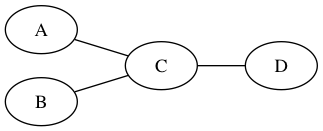
\includegraphics[scale=0.75]{resources/graphviz-dot-example.png}
    \caption{Resultat des Aufrufs des Kommandozeilen-Tools \texttt{dot}}
    \label{fig:graphviz-dot-example}
\end{figure}

Alternativ kann die Dot-Quelldatei in der GUI-Anwendung geöffnet werden. In dem Fall wird das Ergebnis nicht direkt in eine Datei gespeichert, sondern als PDF in einem Fenster der Anwendung angezeigt.

In dem oben diskutierten Beispiel wird sichtbar gemacht, dass das resultierende Diagramm nicht interaktiv ist. Eine Änderung des Graphen ist nur in der Quelldatei möglich und ist mit einem wiederholten Aufruf des Kommandozeilen-Tools oder Laden der Datei in der GUI-Anwendung verbunden. Diese Schwachstelle wird durch 3rd-Party Editoren mit der integrierten grafischen Ausgabe wie etwa \textit{Leonhard}\footnote{\textit{Leonhard} ist ein grafischer Editor für \textit{Graphviz}, der unter älteren Versionen von Mac OS X funktioniert. Weitere Information sind unter \url{http://algorithmique.net/leonhard.html} und \url{https://github.com/glejeune/Leonhard} zu finden.} oder \textit{WebGraphviz}\footnote{\url{http://webgraphviz.com}} verbessert. In \textit{Leonhard} wird die Übersetzung nach jeder Änderung des Quelltexts sogar automatisch gestartet.

Trotz der fehlenden Interaktivität des resultierenden Diagramms kann das Layout von dem Nutzer beeinflusst werden, indem der Layout-Algorithmus gewählt wird bzw. seine Parameter in der Quelldatei angepasst werden \cite{NorthGansner14Dot-Manual}. Im oben genannten Beispiel wurde der Layout-Algorithmus \texttt{dot} verwendet und die Richtung des Graphen in der Dot-Quelldatei mit dem Befehl \texttt{rankdir = LR} angepasst, so dass der Graph von links nach rechts gezeichnet wird.

\subsubsection{Textbasierte UML-Tools}

Neben den textbasierten Tools für das Graphzeichnen gibt es Tools, die für spezifische Domänen ausgelegt sind. Im Folgenden werden 2 textbasierte UML-Tools kurz vorgestellt, die aus einer textuellen Beschreibung in einer speziellen Sprache grafische UML-Diagramme erzeugen. Für die Berechnung des Layouts benutzen beide Tools intern die oben vorgestellte Bibliothek \textit{Graphviz}.

\paragraph{PlantUML}

\hyphenation{PlantUML}

\textit{PlantUML}\footnote{\url{http://plantuml.sourceforge.net}} ist eine Java-Bibliothek, die für die Beschreibung von UML-Diagrammen die gleichnamige Sprache verwendet. Diese Sprache wird näher in \cite{Roques10Drawing} behandelt. Neben den vielen Anwendungen\footnote{Die bekannten Anwendungen sind unter \url{http://plantuml.sourceforge.net/running.html} aufgelistet.} bietet \textit{PlantUML} einen Online-Editor\footnote{\textit{PlantUML} Server: \url{http://www.plantuml.com/plantuml}} an, der es ermöglicht, UML-Diagramme direkt im Browser zu erstellen und als Bilder zu exportieren.

\paragraph{yUML}

\textit{yUML}\footnote{\url{http://yuml.me}} ist ein Online-Editor zum Erstellen von UML-Diagrammen im Browser. Im Unterschied zu \textit{PlantUML} verwendet \textit{yUML} eine anschauliche zeichenbasierte Sprache\footnote{Eine Übersicht der Syntax für Klassendiagramme: \url{http://yuml.me/diagram/scruffy/class/samples}}. Die Eingabe erfolgt über ein Textfeld und wird kontinuierlich in ein Bild übersetzt, das jederzeit exportiert werden kann. Alternativ kann eine URL-Adresse generiert \cite{Fuhrmann11On-the-Pragmatics} werden, unter der das gezeichnete Diagramm online verfügbar ist.

\subsection{Visuelle Ansätze}
\label{subsec:visual-approaches}

Die visuellen Ansätze für das automatische Layout unterscheiden sich von den textbasierten darin, dass der Layout-Algorithmus auf eine visuelle Sprache angewendet wird und dass das berechnete Layout direkt die Eingabe verändert. Diese Ansätze werden in der Regel in visuellen Editoren eingesetzt, die eine unmittelbare Bearbeitung des Diagramms unterstützen.

Der Ablauf ist wie folgt: Zunächst wird ein Diagramm in einer bestimmten visuellen Sprache (z.B. ein Klassendiagramm in der Sprache UML) modelliert. Dann wird ein Layout-Algorithmus (in der Regel manuell) ausgeführt, der das neue Layout für alle Diagrammbestandteile berechnet. Anschließend wird das modellierte Diagramm dermaßen angepasst, so dass es das berechnete Layout annimmt.

Die Entkoppelung der Ein- und Ausgabe, wodurch sich die textuellen Ansätze auszeichnen (siehe Abschnitt \ref{subsec:text-based-approaches}), entfällt an dieser Stelle und da das resultierende Diagramm interaktiv bleibt, kann es durch den Nutzer weiterhin verändert bzw. erweitert werden. Um nach jeder Änderung des Diagramms ein automatisch berechnetes Layout zu erhalten, muss allerdings der Layout-Algorithmus jedes Mal erneut gestartet werden.

Die Algorithmen für das automatische Layout sind im Allgemeinen nicht ideal und die Nutzer neigen dazu, das berechnete Layout für persönliche Präferenzen anzupassen, um ein mentales Modell (siehe Abschnitt \ref{subsec:mental-map}) bzw. eine sekundäre Notation (siehe Abschnitt \ref{subsec:layout-of-a-diagram}) zu verwalten. Alle nachträglich manuell getätigten Layout-Änderungen werden bei einem erneuten Aufruf des Layout-Algorithmus verworfen und somit steht der Nutzer vor der Entscheidung, ob er nach jedem Aufruf des Algorithmus die Anpassungen wiederholt durchführt oder auf das automatische Layout komplett verzichtet \cite[S.119ff]{Eiglsperger04Automatic}.

\subsubsection{Automatisches Layout in OmniGraffle}
\label{subsubsec:omnigraffle-auto-layout}

Wie im Abschnitt \ref{subsubsec:graph-drawing-tools} beschrieben wurde, bietet \textit{Graphviz} eine Software-Bibliothek an, die sich in Programme einbinden lässt. Das Visualisierungsprogramm \textit{OmniGraffle} (siehe Abschnitt \ref{subsubsec:omnigraffle}) macht sich dies zu Nutze und bietet eine Funktion für das automatische Layout an, die Algorithmen aus \textit{Graphviz} für die Layout-Berechnung verwendet, nämlich den hierarchischen, kraftbasierten, zirkulären und radialen Algorithmus \cite{Olsen10OmniGraffle}. Nachdem die Funktion des automatischen Layouts aktiviert wird, kann der Layout-Algorithmus ausgewählt und seine Parameter eingestellt werden\footnote{Die konkreten möglichen Parameter der Algorithmen sind in \cite[S.74]{08OmniGraffle} nachzuschauen.}. In Abbildung \ref{fig:omnigraffle-automatic-layout} wird ein Beispiel der Anwendung von allen verfügbaren Layout-Algorithmen auf ein Diagramm illustriert.

\begin{figure}[hbt]
    \newcommand{\subfigureshortwidth}{0.28\textwidth}
    \newcommand{\subfigurelongwidth}{0.40\textwidth}
    \newcommand{\graphicsscale}{0.7}
    \centering
    \begin{subfigure}{\subfigureshortwidth}
        \centering
        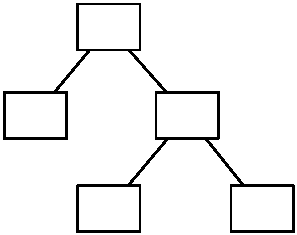
\includegraphics[scale=\graphicsscale]{resources/omnigraffle-automatic-layout-a}
        \caption{Manuell erstelltes Layout}
        \label{fig:omnigraffle-automatic-layout-a}
    \end{subfigure}
    \begin{subfigure}{\subfigureshortwidth}
        \centering
        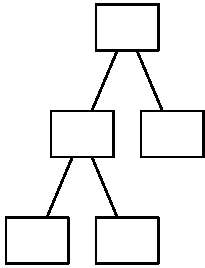
\includegraphics[scale=\graphicsscale]{resources/omnigraffle-automatic-layout-b}
        \caption{Hierarchisches Layout von oben nach unten}
        \label{fig:omnigraffle-automatic-layout-b}
    \end{subfigure}
    \begin{subfigure}{\subfigureshortwidth}
        \centering
        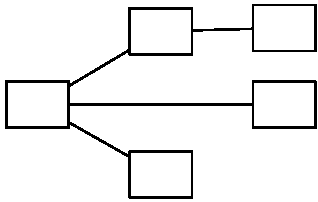
\includegraphics[scale=\graphicsscale]{resources/omnigraffle-automatic-layout-c}
        \caption{Hierarchisches Layout von links nach rechts mit angepassten Ranks für einzelne Knoten}
        \label{fig:omnigraffle-automatic-layout-c}
    \end{subfigure}
    \begin{subfigure}{\subfigureshortwidth}
        \centering
        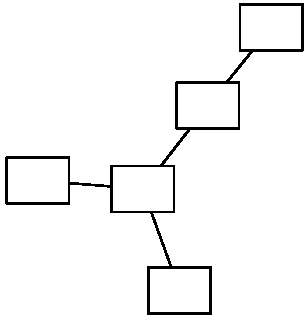
\includegraphics[scale=\graphicsscale]{resources/omnigraffle-automatic-layout-d}
        \caption{Kraftbasiertes Layout}
        \label{fig:omnigraffle-automatic-layout-d}
    \end{subfigure}
    \begin{subfigure}{\subfigurelongwidth}
        \centering
        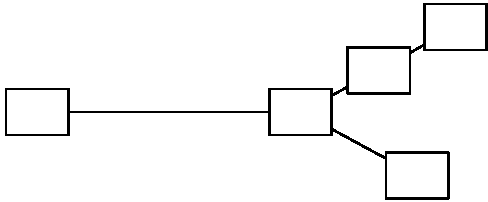
\includegraphics[scale=\graphicsscale]{resources/omnigraffle-automatic-layout-e}
        \caption{Zirkuläres Layout}
        \label{fig:omnigraffle-automatic-layout-e}
    \end{subfigure}
    \begin{subfigure}{\subfigureshortwidth}
        \centering
        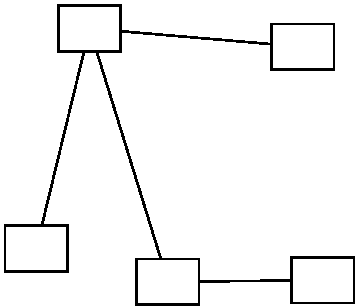
\includegraphics[scale=\graphicsscale]{resources/omnigraffle-automatic-layout-f}
        \caption{Radiales Layout}
        \label{fig:omnigraffle-automatic-layout-f}
    \end{subfigure}
    \caption{Beispiele der Anwendung von automatischen Layout-Algorithmen in OmniGraffle}
    \label{fig:omnigraffle-automatic-layout}
\end{figure}

Der Layout-Algorithmus kann entweder durch die manuelle Auswahl im Menü, die Veränderung der Parametern des Algorithmus oder das Hinzufügen oder Löschen einer Kante zwischen zwei Knoten aufgerufen werden \cite[S.43]{Wybrow08Using}. Danach wird das Layout berechnet und mit Hilfe einer Animation auf das Diagramm angewendet, wobei die vorher durchgeführten manuellen Anpassungen verworfen werden. \textit{OmniGraffle} erweitert die Funktion des automatischen Layouts um weitere Tools. So kann z.B. die Struktur des Diagramms parallel in einer Outline bearbeitet oder ein Werkzeug für schnelle Erstellung eines Diagramms verwendet werden \cite{08OmniGraffle}.

\subsubsection{Automatisches Layout in Visual Paradigm}

% Zusatzfunktion
% semantische Unterstützung fehlt
% manueller Aufruf [Fuhrmann]
% verschiedene Algorithmen -> nur Verbindungen vs. alles

\subsection{Spezielle Algorithmen für Klassendiagramme}

%Eine weitere Gruppe der Ansätze wird durch Algorithmen gebildet, die für das automatische Layout von Klassendiagrammen spezialisiert sind.

%Ähnlich wie die Algorithmen zum Graphzeichnen lassen sich diese Algorithmen in visuelle Editoren einbauen, sind allerdings für eine interaktive Nutzung nicht geeignet. % Eiglsperger beschreibt, wie der Algorithmus zu erweitern ist, um ihn interaktiv einsetzen zu können

% TODO: Speziellen Algorithmen ergänzen!

% Traditionelle Kriterien für Graphzeichnen sind für Klassendiagramme nicht ausreichend [Eichelberger S.79]

% SugiBib - ein Framework, das auf dem Sugiyama Algorithmus basiert und die Semantik und Strukturregeln berücksichtigt
% https://wwwi2.informatik.uni-wuerzburg.de/SugiBib
% XMI (Input siehe Eichelberger 47ff)

% Kandinsky (Eiglsperger)

% im Unterschied zu [Eichelberger] beschäftigt sich diese Arbeit mit interaktiven Ansätzen, da automatisches Layout gegen Agile Modeling verstößt

\subsection{Zusammenfassung der Eigenschaften}

\subsubsection{Vorteile}
% TODO: Diesen Abschnitt überprüfen!

\begin{itemize}
    \item \textbf{Automatische Layout-Berechnung} Das automatische Layout, wie man dem Namen entnehmen kann, wird automatisch berechnet und spart somit die Arbeit an manueller Layout-Erstellung. In der Regel werden optimale Layouts im Bezug auf die ästhetischen Kriterien geliefert \cite{Maier12A-Pattern-based}. Durch die Spezialisierung der Algorithmen kann sogar das Einhalten der Strukturregeln der konkreten Diagrammtypen erreicht werden.
    \item \textbf{Einbinden in automatisierte Prozesse} Aufgrund des statischen Charakters und der definierten Eingabesprachen ist die automatische Layout-Berechnung für das Einbinden in automatisierte Prozesse geeignet. Beispiele dafür sind das automatisierte Generieren von Diagrammen in dem Dokumentations-Tool Doxygen\footnote{\url{http://www.stack.nl/~dimitri/doxygen/manual/diagrams.html}} oder Plugins zum Zeichnen von Diagrammen für Wiki-Seiten.
\end{itemize}

\subsubsection{Nachteile}

\begin{itemize}
    \item \textbf{Fehlende Interaktivität} Das automatische Layout ist für eine interaktive Bearbeitung der Diagramme nicht konzipiert, da die direkte Interaktion des Nutzers mit dem Diagramm mangelhaft oder gar nicht unterstützt wird. Obwohl sich die visuellen Ansätze in interaktiven Umgebungen wie etwa visuellen Editoren einsetzen lassen, sind sie dafür nicht geeignet \cite[S.22ff]{Maier12A-Pattern-based} \cite[S.4]{DwyerMarriott08Interactive}. Insbesondere zeichnet sich dies dadurch aus, dass der Prozess der Erstellung eines Diagramms nicht gefördert wird. Die interaktiven Änderungen des Inhalts bzw. des Layouts des Diagramms werden von dem Layout-Algorithmus nicht berücksichtigt und somit kann bei dem Aufruf des Algorithmus das mentale Modell (siehe Abschnitt \ref{subsec:mental-map}) bzw. die sekundäre Notation (siehe Abschnitt \ref{subsec:layout-of-a-diagram}) zerstört werden \cite{Eiglsperger04Automatic}. Des Weiteren ist es notwendig, den Algorithmus manuell nach jeder Änderung erneut zu starten. Im Unterschied zu den visuellen Ansätzen bieten die textuellen Ansätze keine direkte Form der Interaktion an, was durch die unterschiedlichen Eingabe- und Ausgabesprachen und der damit zusammenhängenden Entkoppelung der Eingabe und Ausgabe bedingt ist.
    \item \textbf{Geringer Einfluss auf das Layout} Da das automatische Layout auf statischen Algorithmen basiert, die sich in der Regel nur durch die Anpassung der Parameter beeinflussen lassen, werden die Layout-Präferenzen des Nutzers nicht berücksichtigt. Die mögliche Kontrolle des Ergebnisses des Layout-Prozesses ist somit sehr mangelhaft \cite[S.382]{GladischSchumann14Semi-Automatic}.
    \item \textbf{Mangelhafte Berücksichtigung der Syntax- und Semantikregeln} Die syntaktischen und semantischen Layout-Regeln der konkreten Diagrammtypen werden von den allgemeinen Algorithmen für das Layout von graphbasierten Diagrammen nicht berücksichtigt und können dadurch verletzt werden.
\end{itemize}

\section{Interaktives halbautomatisches Layout}
\label{sec:interactive-semi-automatic-layout}

Wie bereits in diesem Kapitel präsentiert wurde, unterstützen die meisten Editoren zur Erstellung von Diagrammen Hilfefunktionen für das manuelle Layout (Abschnitt \ref{sec:manual-layout}) und eventuell auch automatische Layout-Algorithmen (Abschnitt \ref{sec:automatic-layout}). Das manuelle Layout ist sehr intuitiv, zeichnet sich durch die direkte Interaktion des Nutzers mit dem Diagramm aus, vermisst aber eine automatisierte Layout-Berechnung und Berücksichtigung der ästhetischen Prinzipien. Dieses Problem wird durch das automatische Layout bekämpft, das aber in dem Bereich der Interaktivität versagt \cite{GladischSchumann14Semi-Automatic}. Die Vorteile der Ansätze aus beiden genannten Kategorien lassen sich kombinieren und bilden eine neue Kategorie der Ansätze für die halbautomatische Layout-Unterstützung.

Diese Ansätze sind für Nutzer-bedingte Änderungen ausgelegt und ermöglichen eine inkrementelle Erstellung der Diagramme mit Bezug auf das Layout. Somit sind sie insbesondere für interaktive Umgebungen geeignet \cite{Arvo02Techniques, GladischSchumann14Semi-Automatic, Wybrow08Using}.


% dynamische Algorithmen, Sequenzen von Modifizierungen
% Nutzer kann einige Aspekte des Layouts beeinflussen, z.B. durch direkte Positionierung der Knoten bzw. Kanten oder durch eine Form von Feedback [Arvo02]
% inkrementelles Layout

\subsection{Struktur-basierte benutzergesteuerte Ansätze}
\label{subsec:structure-based-user-controlled-approaches}

Die erste Kategorie der Ansätze für das interaktive halbautomatische Layout bilden die Struktur-basierten benutzergesteuerten Ansätze, die dem Nutzer ermöglichen, das Layout des Diagramms durch Erstellung und Verwaltung von Strukturregeln\footnote{Ein Beispiel für eine solche Strukturregel ist die im Abschnitt \ref{subsubsec:alignment-and-distribution} beschriebene gleichmäßige Verteilung der ausgewählten Objekte in Relation zueinander.} zu beeinflussen. Diese Strukturregeln erinnern an die Hilfefunktionen für das manuelle Layout (siehe Abschnitt \ref{subsec:help-functions-for-manual-layout}), sind aber dahingegen persistent \cite{Wybrow08Using}. Sie werden bei der Berechnung des Layouts durch einen dynamischen Layout-Algorithmus berücksichtigt und eingehalten.

Die Struktur-basierten benutzergesteuerten Ansätze lassen sich in zwei Gruppen unterteilen: in Constraint-basierte und Pattern-basierte Ansätze. Beide Gruppen werden im Folgenden vorgestellt.

\subsubsection{Constraint-basierte Ansätze}
\label{subsubsec:constraint-based-approaches}

Die Strukturregeln können mit Hilfe von Constraints umgesetzt werden. Ein valides Layout wird dadurch berechnet, indem alle Constraints im Diagramm mit einem Constraintlöser ausgewertet werden.



% deklarativ
% welche Regeln sollen gelten anstatt wie
% Constraintlöser, verschiedene Typen (beschrieben in [Mai])

% Cassowary for layout of UI in Cocoa/iOS

% Dunnart: Screenshot, http://dunnart.org
% Nutzer kann Constraints erstellen und auf Teile des Diagramms anwenden

% Probleme mit der Performance, da der Algorithmus nach jeder kleinen Änderung laufen muss

\subsubsection{Pattern-basierter Ansatz}
\label{subsubsec:pattern-based-approach}

Der in \cite{Maier12A-Pattern-based} und \cite{MaierMinas10Combination} präsentierte Pattern-basierte Ansatz für das Layout von Diagrammen drückt die Strukturregeln in Form von Layout-Patterns aus. Der Ansatz kann für beliebige visuellen Sprachen eingesetzt werden, die mit Metamodellen beschrieben werden können. Dabei besteht das sprachenspezifische Metamodell aus zwei Teilen, nämlich der Metamodelle für die abstrakte und konkrete Syntax. Das zuletzt genannte Metamodell beschreibt die visuellen Eigenschaften der Sprache und wird daher durch die Berechnung des Layouts beeinflusst.

Die Beschreibung der Layout-Patterns erfolgt allerdings nicht mit Hilfe der sprachenspezifischen Metamodellen, sondern mit sprachenunabhängigen Pattern-spezifischen Meta-Model\-len\footnote{In \cite{Maier12A-Pattern-based} werden u.a. Pattern-spezifische Metamodelle für Mengen von Elementen, geordnete Listen von Elementen oder Graphen vorgestellt.}. Bei der Instanziierung eines Layout-Patterns wird das sprachenspezifische Modell auf ein Pattern-spezifisches Modell abgebildet\footnote{Dieses Sachverhalt wird mit Hilfe eines Beispiels in \cite[S.59ff]{Maier12A-Pattern-based} anschaulich gemacht.}. Dadurch wird eine mögliche Wiederverwendung der Layout-Patterns für diverse visuellen Sprachen gewährleistet. Weiterhin zeichnet sich der Pattern-basierte Ansatz dadurch aus, dass die Layout-Patterns verschiedene Ansätze zum Layout von Diagrammen u.a. Algorithmen zum Graphenzeichnen (siehe Abschnitt \ref{subsubsec:graph-drawing-tools}) und Constraints-basierte Algorithmen (siehe Abschnitt \ref{subsubsec:constraint-based-approaches}) kombinieren und sich zunutze machen.


% Auflistung der Layout-Patterns: tree layout, layered layout, equal distance, alignment…

%Kontroll-Algorithmus läuft im Hintergrund nach jeder Änderung des Diagramms bzw. der Instanziierung eines Layout-Patterns

% benutzergesteuert, nicht eingeschränkt in Interaktion

%Wie bereits erwähnt, ist dieser Ansatz für interaktive


% Videos: http://www.sonjamaier.de/dyndraw/screencasts/graphEditor.mov & http://www.sonjamaier.de/dyndraw/screencasts/ecoreEditor.mov

Dieser Ansatz wurde in Form eines Layout-Frameworks\footnote{\url{http://www.unibw.de/inf2/Personen/Wissen_Mitarbeiter/sonja/research/layoutframework}} implementiert, das bisher nicht veröffentlicht wurde. Dennoch wurde es in visuellen Editoren eingesetzt, die mit Hilfe von DiaMeta\footnote{Ein Framework zur Generierung von Editoren für visuelle Sprachen basierend auf Spezifikationen mittels Metamodelle. \url{http://www.unibw.de/inf2/DiaGen/}} bzw. Graphical Editing Framework\footnote{\url{http://www.eclipse.org/gef/}} erzeugt wurden \cite{Maier12A-Pattern-based}.

\subsection{Anwendungsspezifische Ansätze}

Die Struktur-basierten benutzergesteuerten Ansätze für das halbautomatische Layout, die im Abschnitt \ref{subsec:structure-based-user-controlled-approaches} beschrieben wurden, sind sehr universell und können in Editoren für verschiedene visuellen Sprachen eingesetzt werden. Aus diesem Grund können die syntaktischen und semantischen Eigenschaften der Sprachen nicht gründlich in den Algorithmen berücksichtigt werden. Dahingegen gibt es anwendungsspezifische Ansätze, deren Algorithmen für konkrete visuelle Sprachen entworfen sind. Diese werden im Folgenden vorgestellt.

\subsubsection{Smart Layout in MindNode}
\label{subsubsec:smart-layout-in-mindnode}

\textit{MindNode}\footnote{\url{https://mindnode.com}} ist eine benutzerfreundliche Desktop-Anwendung zur Erstellung von Mind-Maps für Mac OS X. Die Mind-Maps haben eine baumbasierte Struktur mit einem oder mehreren zentralen Knoten. Weiterhin gilt, dass jeder Knoten mehrere Unterknoten besitzen kann und alle Knoten außer den zentralen Knoten genau einen Oberknoten haben. Die hierarchischen Relationen werden mit farbigen Zweigen dargestellt. Zusätzlich bietet \textit{MindNode} die Möglichkeit der Querverbindungen zwischen Knoten aus unterschiedlichen Teilen der Mind-Map, die mit gestrichelten Pfeilen gekennzeichnet werden \cite{14MindNode}. In Abbildung \ref{fig:mindnode-example} ist ein Beispiel einer Mind-Map zu sehen.

\begin{figure}[hbt]
    \centering
    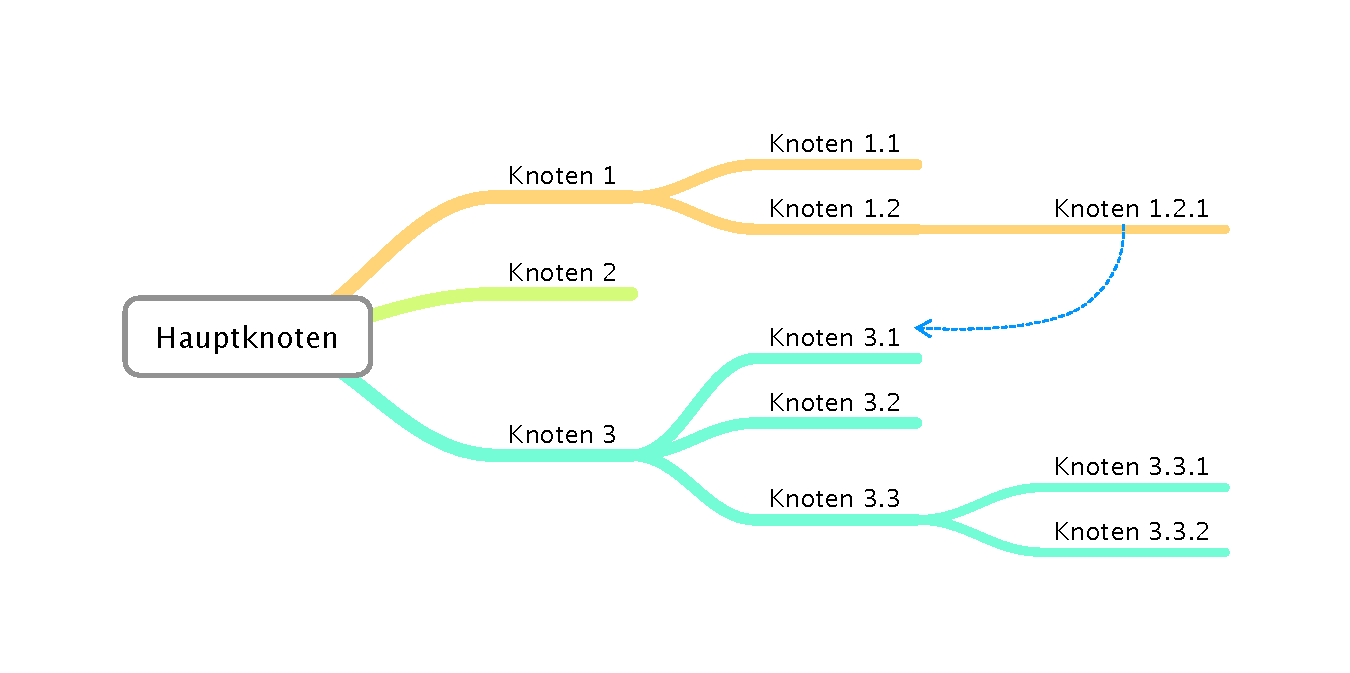
\includegraphics[
        width=\textwidth,
        trim={0 1.5cm 0 1.5cm},
        clip
    ]{resources/mindnode-example}
    \caption{Beispiel einer Mind-Map in \textit{MindNode}}
    \label{fig:mindnode-example}
\end{figure}

\textit{MindNode} stellt eine interaktive Funktion für eine halbautomatische Layout-Unterstützung namens \enquote{Smart Layout} bereit \cite{14MindNode}. Wenn diese Funktion ausgeschaltet ist, können einzelne Knoten der Mind-Map frei positioniert werden. Dahingegen, wenn die Funktion eingeschaltet ist, nimmt die Mind-Map eine vorgerechnete Baumstruktur an und die Verschiebungsoperation eines Knotens drückt in diesem Fall die Absicht einer Layout-Modifikation aus.

In Abbildung \ref{fig:mindnode-smart-layout} wird die Funktionsweise der Funktion \enquote{Smart Layout} anhand von Screenshots gezeigt. Zunächst wird in \ref{fig:mindnode-smart-layout-a} ein Knoten angeklickt, dessen Position angepasst werden soll. Mit \enquote{Drag and Drop} wird in \ref{fig:mindnode-smart-layout-b} der Knoten auf die gewünschte Position verschoben. Die Verbindung zu dem Oberknoten wird dabei mit einem helleren Zweig veranschaulicht. Nach dem Loslassen der Maustaste in \ref{fig:mindnode-smart-layout-c} wird die gewünschte Position der verschobenen Knotens ausgewertet, ein neues Layout der Mind-Map anhand des Hinweises durch die Verschiebungsoperation berechnet und anschließend auf die Mind-Map angewendet, indem alle beeinflussten Knoten von ihren aktuellen Position zu ihren neuen Position animiert werden. Somit kann der Nutzer das Layout beeinflussen, wird aber in den Möglichkeiten eingeschränkt. Dies führt in der Regel zu einem optimalen Layout und ist vor allem durch die Struktur der visuellen Sprache für Mind-Maps möglich.

% Unterknoten des zentralen Knotens können auf die linke bzw. rechte Seite verschoben werden
% initiales Layout

\begin{figure}[hbt]
    \newcommand{\subfigurewidth}{\textwidth}
    \newcommand{\graphicswidth}{0.7\linewidth}
    \begin{subfigure}{\subfigurewidth}
        \centering
        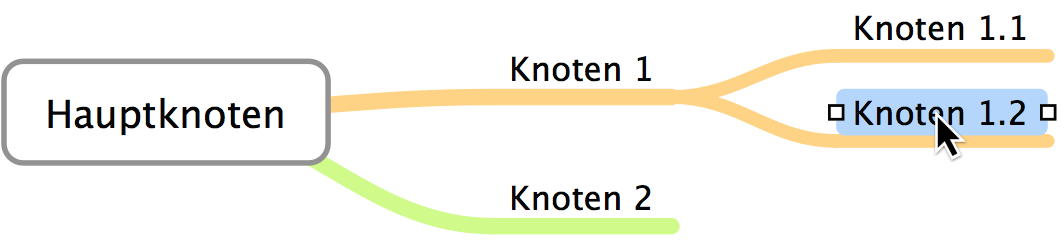
\includegraphics[width=\graphicswidth]{resources/mindnode-smart-layout-a}
        \caption{}
        \label{fig:mindnode-smart-layout-a}
    \end{subfigure}
    \begin{subfigure}{\subfigurewidth}
        \centering
        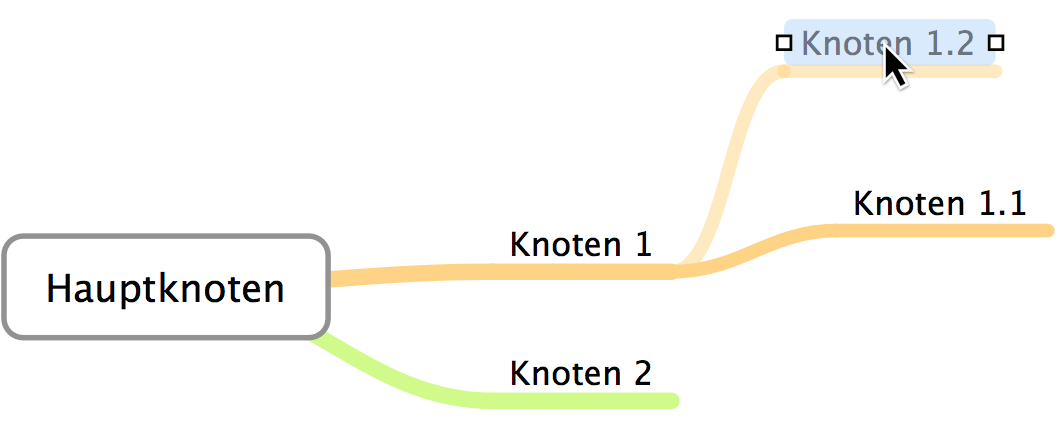
\includegraphics[width=\graphicswidth]{resources/mindnode-smart-layout-b}
        \caption{}
        \label{fig:mindnode-smart-layout-b}
    \end{subfigure}
    \begin{subfigure}{\subfigurewidth}
        \centering
        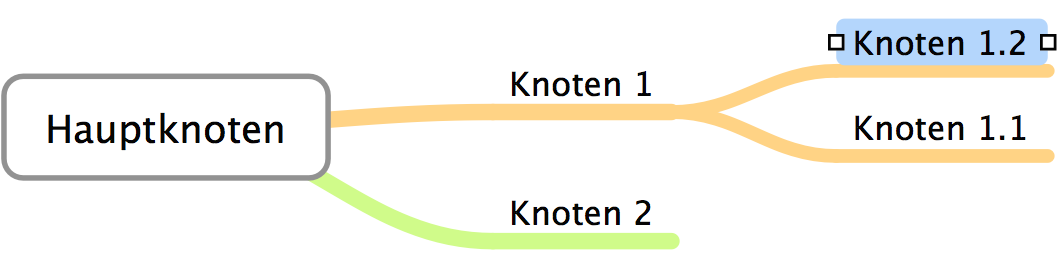
\includegraphics[width=\graphicswidth]{resources/mindnode-smart-layout-c}
        \caption{}
        \label{fig:mindnode-smart-layout-c}
    \end{subfigure}
    \caption{Eine Verschiebungsoperation mit der eingeschalteten Funktion \enquote{Smart Layout} in \textit{MindNode}}
    \label{fig:mindnode-smart-layout}
\end{figure}

\subsection{Zusammenfassung der Eigenschaften}

% Wahrnehmungsorganisation hat eine größere Priorität als reine Berücksichtigung der syntaktischen Ästhetik [Shieber]
% Beides Kombinieren [Shieber]

% Nur visualisieren vs. auch Editieren [Gladisch]
% Nutzer entwickeln ein mentales Modell des Diagramms, das soll bei den inkrementellen Updates berücksichtigt werden [Gladisch]

% Der Nutzer kann das Diagramm unmittelbar bearbeiten
% das mentale Modell bleibt beibehalten [preserving the mental map (in dynamic context) instead of aesthetics (in static context)]
% ästhetische Regeln werden nicht eingehalten

% ZUSAMMENFASSUNG
% Tabelle für den Vergleich zwischen den bestehenden Ansätzen und meinem Ansatz
